\pagenumbering{arabic}
\section{绪论}

\subsection{研究背景及意义}
\subsubsection{研究背景}

医学图像是指利用医学成像技术生成的视觉图像,涵盖计算机断层扫描(CT)、磁共振成像(MRI)、超声成像(US)等多种成像模态,通过分析其提供的组织结构、解剖细节及病理信息,放射科医师和内科医师可以快速准确地进行医疗诊断。对医学图像进行图像分割是分析的关键步骤之一,它涉及将图像划分为解剖结构或病灶区域(如器官、组织或病变)相对应的不同区域,这种支持肿瘤定位、器官边界划定的分割可以精确解释医学图像,为临床应用中的准确诊断、术前规划和定量分析奠定了基础\cite{panayides2020}。鉴于其重要性和对临床结果的直接影响,医学图像分割的准确性成为现代医疗健康系统工作中不可或缺的要求。然而,当前临床实践中大量依赖放射科医生手动标注分割图像,不仅耗时费力,还存在一定的主观性和一致性问题。尤其在高分辨率三维图像中,手动标注的工作量极大,容易引发标注者疲劳、遗漏或偏差,进而影响诊断质量。因此,伴随着医学图像数量的激增,研究高效、自动化且高精度的医学图像分割方法,不仅能偶减轻医生负担、提升标注一致性,更在促进智能辅助诊疗系统落地中扮演着不可替代的角色。

\begin{figure}[h]
    \centering
    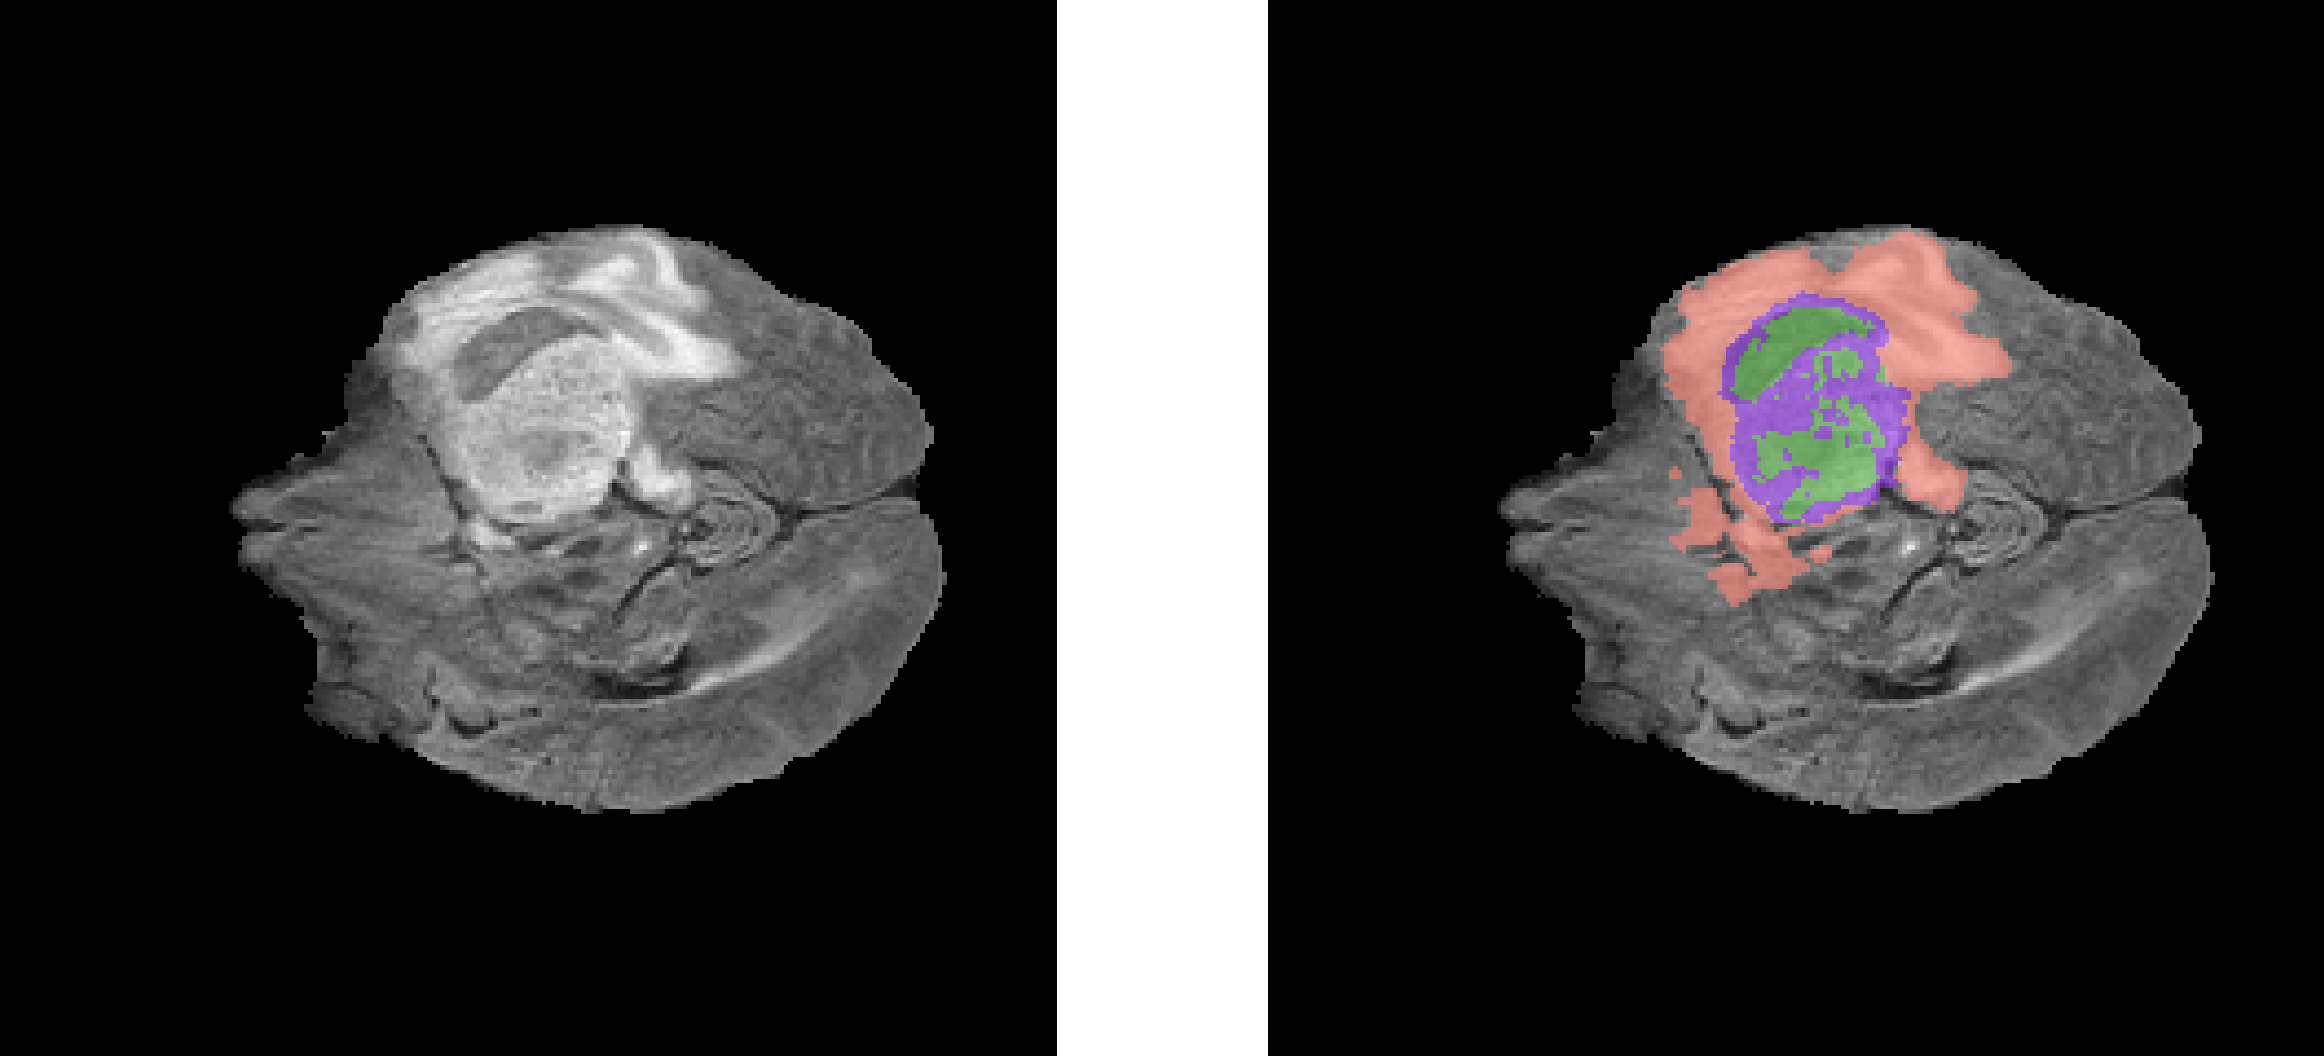
\includegraphics[width=0.77\textwidth]{fig/flair_and_mask.png}
    \caption{脑部MRI图像(左)及对应肿瘤手工标注结果(右)}
    \label{brian_tumor}
\end{figure}

在医学图像分割的发展早期,主要利用阈值分割、区域生长、边缘检测、聚类分割等传统算法进行组织、器官及病灶区域的识别与提取。这些方法大多依赖人工设计特征或强先验假设,基于像素灰度、边缘梯度、区域一致性等低层视觉信息构建规则,具有较高的可解释性和计算效率。然而,面对实际医学影像数据的复杂性,这些方法暴露出明显的局限性。医学影像中常见的解剖结构形态复杂、边界模糊(如肿瘤与周围组织过渡不清)、组织密度差异微弱,使得依赖简单灰度或梯度判断的传统方法难以准确建模区域间差异。此外,医学影像中的特殊挑战进一步削弱了传统方法的泛化能力与适应性:包括成像过程中引入的噪声干扰、患者间器官形态的个体差异与非线性形变、边界信息的不确定性、以及多模态成像之间强度分布的显著差异\cite{mohdsagheer2020}。这些因素对传统算法构成了严峻挑战,使其在跨患者、跨设备或跨模态应用中难以保持一致性能。同时,在临床实际应用中,常需依赖专业人员进行参数调整、种子点选择或后处理操作,操作流程繁琐、效率低下,严重制约了其在大规模医学影像分析系统中的推广与部署。基于上诉原因,尽管传统图像分割方法在特定条件下仍具参考价值,但其在面对复杂医学图像时的表达能力与适应性显然不足,亟需更具自动学习能力和结构建模能力的先进方法来突破其局限。

随着神经网络及深度学习的迅速发展和应用,以卷积神经网络为代表的深度学习方法在图像分类、检测与分割等计算机视觉任务中取得了突破性进展,其端到端的特征提取能力和强大的表征学习能力,使得图像分割任务由传统手工设计特征的范式,转向自动特征学习与高维特征建模的方向。而最早将深度学习应用于图像分割的代表性模型包括全卷积神经网络与SegNet等。全卷积神经网络通过去除全连接层,将图像映射为像素级别的类别预测图,是端到端分割网络的开端\cite{shelhamer2016};SegNet在其基础上引入池化索引进行上采样,提升了细节还原能力。至此,利用卷积神经网络等技术,深度学习方法凭借其优异的图像分割性能和适应性,在医学图像分割领域逐渐取代了传统算法的地位。然而,这些早期模型在医学图像场景下仍面临着一定局限:如对弱边界区域识别不敏感,对结构复杂或形变剧烈的解剖区域分割精度有限,且对小样本训练数据依赖较强,泛化能力不足等。

为应对医学图像小样本、边界模糊等挑战,Ronneberger等人\cite{ronneberger2015}于2015年提出了经典的U-Net模型,成为了医学图像分割领域的里程碑。U-Net采用编码器-解码器结构,前半部分通过卷积与池化提取高层语义特征,后半部分通过反卷积逐步还原空间分辨率。同时,网络在对称位置引入跳跃连接,将编码器中浅层的高分辨率特征与解码器中对应层的特征图进行拼接融合,从而有效弥补了深层语义特征中局部细节的丢失,实现了多尺度特征的整合与边界定位能力的增强。在ISBI细胞分割挑战赛中,U-Net凭借其出色的结构设计,以显著优势获得冠军。这一成功也推动了U-Net成为后续医学图像分割研究的基准模型,被广泛应用于脑肿瘤、乳腺癌、肺部病灶、眼底血管、皮肤病变等多种应用场景,并衍生出众多变体。U-Net的提出不仅标志着深度学习在医学图像分割领域的广泛应用起点,也为融合传统知识与深度模型提供了范式基础,奠定了现代医学图像分割算法的主流框架。

\begin{figure}[h]
    \centering
    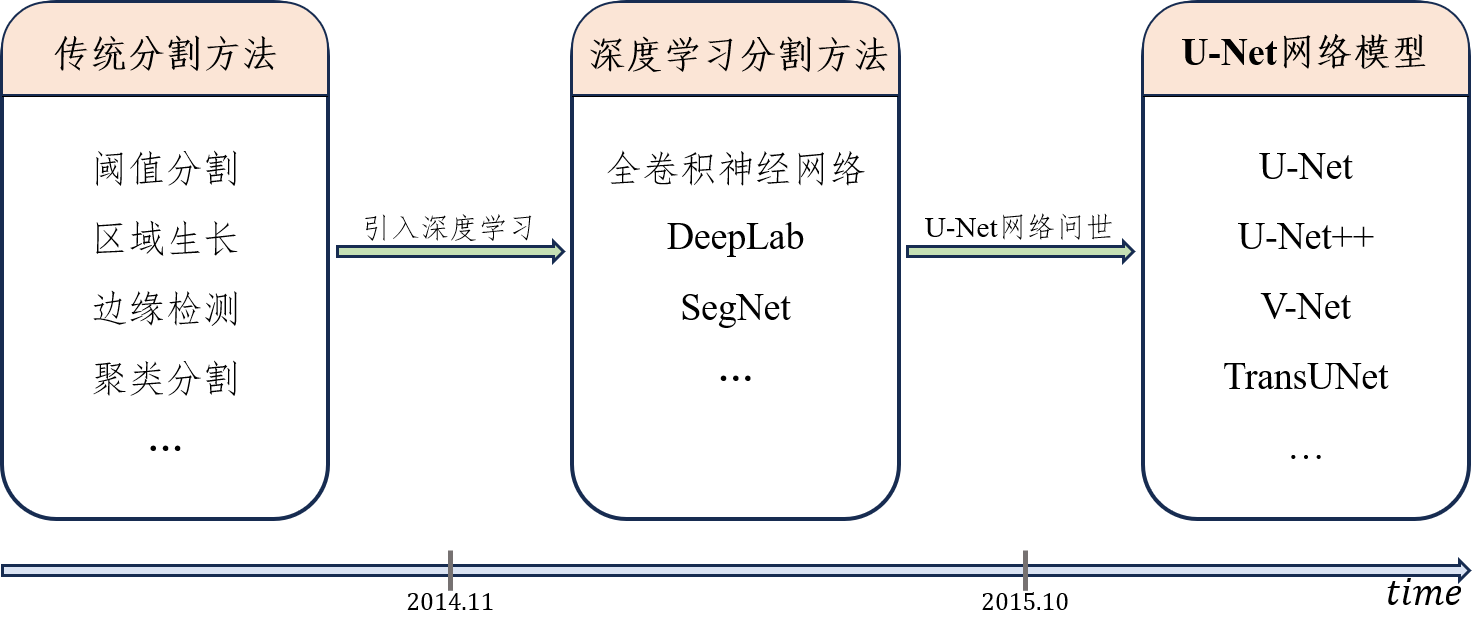
\includegraphics[width=\textwidth]{fig/develepment_of_seg.png}
    \caption{医学图像分割方法发展脉络}
    \label{develop_seg}
\end{figure}

尽管U-Net在医学图像分割中取得了巨大的成功,但随着临床场景的复杂化与精度需求的提高,原始U-Net在多种实际应用中仍存在显著局限性。首先,在多目标重叠、边界模糊或形态不规则的复杂场景中,U-Net的分割准确性容易下降。例如,面对多个病灶区域相互接近或重叠(如多发性肿瘤、血管交叉结构)时,模型难以有效区分各目标,易发生融合或漏检现象;对于尺寸较小的病灶(如早期病变、微小转移灶),因其在特征图中易被下采样过程压缩甚至丢失,导致分割结果中频繁出现漏检;此外,U-Net对输入图像质量也较为敏感,在存在伪影、噪声或成像伪差等干扰时,模型的鲁棒性难以保证\cite{azad2024}。

随着医疗影像技术的不断发展和临床需求的日益提升,医学图像分割任务面临着更高层次的挑战与期望。传统的二维静态图像处理已难以满足当前复杂的医学场景,特别是在涉及动态器官(如心脏、肺部)或介入手术导航等实时性强的应用中,分割模型不仅需要具备快速响应能力,还要在保持精度的同时实现高效率推理。此外,随着三维成像技术的普及,诸如CT、MRI等医学影像数据普遍具有体积属性,甚至在某些应用中演化为四维(随时间变化的3D序列)数据,这对模型提出了在空间与时间维度上同时建模的能力要求。因此,支持3D/4D数据结构处理已成为医学图像分割发展的重要方向。

针对上述高阶需求,现有研究虽已在多个方向取得一定进展,但仍存在明显空白,特别是如何针对具体医学应用场景对U-Net进行定制化改进的问题仍缺乏系统探索\cite{krithikaaliasanbudevi2022}。例如,对于多模态影像(如PET-CT、T1/T2-weighted MRI等)带来的信息互补特性,如何在U-Net结构中引入多模态融合机制,以提升模型对异构数据间语义关联的建模能力。此外,在实际临床环境中,分割模型常需部署于移动端、边缘设备或术中设备中运行,受限于算力、内存及功耗等资源约束,因此U-Net结构的轻量化设计亦成为关键研究方向之一,如采用深度可分离卷积、网络剪枝、知识蒸馏等手段减小模型体积和计算量,而不显著损失精度。总体而言,如何在保持U-Net核心优势的基础上,围绕注意力建模、多源信息融合与计算效率优化等维度进行针对性设计,构建适用于多样医学场景的高效、稳健、可解释的新型分割模型,是当前研究中亟需填补的重要空白。

\subsubsection{研究意义}

本研究的学术意义主要体现在三个方面:

从理论价值层面出发,对U-Net模型进行系统性改进,提升其对复杂结构、细粒目标及低对比度区域的建模能力,不仅有助于解决医学图像分割中的多个核心难题,也为设计具备更强表达能力与泛化能力的深度模型提供新的思路。而改进后的模型架构及训练策略在结构设计、信息流建模及优化方法等方面均具有一定的创新性,对医学图像语义分割任务的理论体系形成补充,也为应对小样本条件下的训练、提升模型鲁棒性及解释性等问题提供了具有借鉴价值的解法。

从应用价值层面出发,在实际临床中,医学图像分割是许多关键诊疗环节的基础,尤其在肿瘤检测、器官分割、病灶定量评估等任务中具有核心地位。提高分割模型的精度与效率,可有效辅助医生快速准确地定位病灶区域(如脑肿瘤、乳腺结节、血管斑块等),减少漏诊误判,提升诊断一致性,显著缓解医生的工作负担。特别是在多目标重叠、边界模糊等复杂场景中,基于改进U-Net的高性能模型可为医生提供更清晰、准确的辅助分割结果,提升临床诊疗的整体质量。同时,高质量的自动分割模型可广泛应用于放射治疗中的靶区勾画、术前路径规划、术中导航与术后评估中,减少对经验丰富医生的高度依赖,降低因人工勾画不一致带来的手术误差与放疗剂量偏差,为治疗过程的标准化与精细化提供技术保障。此外,结合患者的个体影像特征与多模态医疗数据,本研究成果也将为实现个性化医疗提供支持,如用于移植器官体积与形状评估、疗效追踪、慢病进展预测等,有助于推动以患者为中心的精准医疗落地。

从社会价值层面出发,根据WHO《世界健康统计2025》报告\cite{who2021stats},2023年全球医疗人员缺口高达1470万人,预计2030年仍将维持在1110万人以上,尤其是在非洲与东地中海占据近七成。这一结构性短缺为医学图像自动化分割等智能化辅助技术在全球范围内的应用提供了迫切现实背景,面向基层医疗或资源匮乏地区,轻量化、高精度、可部署性的医学图像分割模型可构建低成本的智能辅助诊断系统,缓解医资不均、专家短缺等公共卫生难题,推动普惠医疗的发展。因此,本研究不仅具备显著的学术理论价值,也具有广泛而深远的临床实践与社会应用前景。


\subsection{国内外研究现状}

自2015年Ronneberger等人提出U-Net以来,被引用超过73600次,其凭借高效的特征提取与恢复能力,在医学影像的任务中取得了广泛的应用,成为了医学图像分割领域最广泛使用的架构之一。然而,传统U-Net仍然存在显著的局限性:在全局信息建模和边界细化方面不足;感受野有限,难以捕捉全局上下文,对结构复杂或背景噪声大的区域理解不足;模型冗余大,计算成本高等。因此,近年来国内外学者针对这些问题以及不同的应用场景,在原始U-Net网络的基础上,通过优化结构、引入注意力机制、融合多尺度特征等方法,提出了多种改进模型。这些改进已在多篇相关综述类文章中被系统总结\cite{azad2024,krithikaaliasanbudevi2022,wang2023},下文中将根据Azad等人提出的U-Net变体分类法\cite{azad2024},对国内外学者的研究现状进行概述。

\subsubsection{国外研究现状}

当前国际学术界在医学图像分割领域主要围绕U-Net架构的改进与创新展开研究,重点研究方向包括:多尺度特征融合优化、混合架构创新和多模态处理突破。

多尺度特征融合策略可以通过组合来自不同空间分辨率或感受野范围的特征,增强网络对不同大小、模糊边界目标的识别能力。因此,许多改进模型通过改进U-Net网络的跳跃连接以增强U-Net网络的多尺度特征融合,以提高其上下文建模能力。Zhou等人\cite{zhou2018}提出了Unet++模型,通过密集跳跃连接优化特征重用,相较于U-Net网络只融合同层级的编码器和解码器特征图,UNet++实现了更精细的多尺度特征融合,改善了小目标与弱边界的分割性能。OKtay等人\cite{oktay2018}最早将注意力机制引入U-Net,通过在跳跃连接中引入注意力门(Attention Gates, AGs),他们提出了attention U-Net模型。attention U-Net可以根据高层语义信息和浅层特征图联合计算注意力权重,增强对目标区域的响应抑制无关区域的响应,同时避免冗余的模型结构。通过在跳跃连接中引入双向卷积LSTM(long-term-short-term-memory)模块,Azad等人\cite{azad2019}提出了BCDU-Net模型,将来自编码器和解码器的特征图在双向卷积LSTM中进行组合,提供了丰富的同时包含语义和局部信息的特征图。

在对称的编码-解码器结构中,通过编码器提取多层次语义特征并压缩空间信息,解码器逐步恢复分辨率并融合浅层细节,可以实现对目标区域的精准分割。相较于U-Net采用卷积神经网络作为编码-解码结构层,许多研究者通过采用或结合不同的网络层来构建U-Net,以提高网络的语义分割能力。受残差网络的启发,Drozdzal等人\cite{drozdzal2016}提出了residual U-Net网络,包含编码-解码层的长跳跃连接和卷积网络层之间跨层的短跳跃连接,实现了相较于原始U-Net网络更快的训练收敛。同样的,Milletari等人\cite{milletari2016}提出了采用3D残差块作为网络主体的V-Net模型,能够实现对3D图像更快更精确的分割。Ibtehaz等人\cite{ibtehaz2020}提出的MultiResUnet则基于Inception块,通过并行堆叠3×3、5×5和7×7卷积核捕获多尺度特征,在保持参数效率的同时,显著提升了模型对多尺寸目标的适应性。此外,Karaali等人\cite{karaali2022}利用密集残差块提出了Residual Dense-Net(RDN),使得特征在局部密集连接中传播的同时,也具备跨单元的残差路径,提升了模型表达能力和训练稳定性。

% 补充例子
位于编码器和解码器中间最底层的瓶颈区域(Bottleneck)代表了输入数据最深层的语义,其分辨率最低通道数最多,对整体性能影响极大。因此,许多研究通过增强瓶颈区域来提升模型对复杂结构的建模能力,弥补压缩造成的信息损失。其中,许多研究者选择引入注意力机制。例如,Guo等人\cite{guo2021}通过在Bottleneck区域引入空间注意力模块(Spatial Attention Module)提出了SA-UNet模型,其设计兼顾性能提升和计算效率,尤其适合处理低信噪比、高结构复杂性的医学图像。

近年来,Transformer模型在自然语言处理(Natural Language Processing, NLP)中表现优异,受此启发,不少研究者将Transformer模型引入至视觉识别任务中。Chen等人\cite{chen2021}在U-Net网络的编码器中引入ViT(Viision Transformer)模型,通过图像化嵌入提取全局上下文谢谢,同时保留卷积神经网络增强局部特征,一定程度上弥补了U-Net对长距离依赖建模能力的不足。Azad等人\cite{azad2022}则利用ViT的全局信息增强的特点,提出了contextual attention network(TMU)模型,通过自适应地融合U-Net生成的局部特征与ViT的全局信息,增强医学图像中重叠边界区域的分割效果。

为了获得丰富的特征表示,医学图像分割领域常用的方法是多尺度与多模态方法。其核心目标在于通过综合利用多模态或多尺度图像中的全部可用信息,同时保留最理想且相关的特征,从而提升训练模型的性能。Dolz\cite{dolz2018}等学者在Dense Multi-path U-Net中提出的创新架构,通过模态融合和Inception模块扩展两方面增强了传统U-Net的丰富表征学习能力,解决了传统多模态分割中早期和晚期融合无法充分建模模态间复杂关系的问题。除此之外,Lachinov等人\cite{lachinov2019}提出的Cascaded Unet通过并行多编码器架构,实现了多模态MRI数据的模态特异性特征提取,克服了原始U-Net对多模态数据同质化处理的局限性。

\begin{table}[!htbp]
  \centering
  \caption{U-Net变体模型的国外改进策略对比}
  \label{tab:unet_var_en}
  \small
  \begin{tabularx}{\textwidth}{@{}C C C@{}}
    \toprule
    \textbf{U-Net变体类别}  
      & \textbf{模型名称} 
      & \textbf{核心改进} \\ 
    \midrule
    \multirow{3}{*}{跳跃连接改进} 
      & UNet++ & 密集跳跃连接跨层级特征融合 \\ \cmidrule(lr){2-3}
      & Attention U-Net & 跳跃连接中嵌入注意力门 \\ \cmidrule(lr){2-3}
      & BCDU-Net & 双向卷积LSTM模块特征融合 \\
    \midrule
    \multirow{4}{*}{主干网络改进} 
      & Residual U-Net & 采用残差块进行长短跳跃连接 \\ \cmidrule(lr){2-3}
      & V-Net & 采用3D残差块处理3D数据 \\ \cmidrule(lr){2-3}
      & MultiResUnet & 采用多尺度并行卷积核 \\ \cmidrule(lr){2-3}
      & RDN & 采用密集残差跨单元路径 \\  
    \midrule
    \multirow{2}{*}{混合Transformer架构} 
      & TransUNet	& 编码器引入ViT提取全局信息 \\ \cmidrule(lr){2-3}
      & TMU & 融合ViT与U-Net特征增强边界 \\
    \midrule
    \multirow{2}{*}{多层次特征增强}
      & Dense Multi-path U-Ne & 多模态融合结合Inception结构 \\ \cmidrule(lr){2-3}
      & Cascaded U-Net & 并行多编码器提取模态特征 \\
    \bottomrule
  \end{tabularx}
\end{table}

综上所述,可以发现,国外医学图像分割研究在算法的创新性、数据资源丰富度及跨学科合作的紧密性等方面表现出明显优势。研究者尝试将Transformer、注意力机制、多模态融合等最新技术融入UNet结构中,不断突破传统模型的局限。但是,国外研究在某些复杂场景下仍存在明显不足,例如对多器官重叠、小病灶等困难场景的分割仍具挑战性,且现有模型在临床应用中的可解释性不足,难以清晰展示决策依据,这成为未来医学图像分割领域的重要发展方向。总体而言,国外的研究持续深入地推动着医学图像分割领域的发展,不断丰富方法论与实践经验,为医学人工智能的发展奠定了坚实基础。

\subsubsection{国内研究现状}

近些年,国内研究者紧跟国际研究的步伐,积极探索U-Net模型改进与应用落地,提出了大量的创新模型及改进方法,主要围绕多尺度特征融合、混合架构设计和轻量化应用三大方向展开创新,兼具理论突破与实际价值。

在U-Net++模型的基础上,Huang等人\cite{huang2020}提出了U-Net3+模型,通过全尺度跳跃连接实现全尺度特征融合显著提高了小目标和模糊边界的识别精度。而Li等人\cite{li2020}提出的Attention U-Net++模型则在U-Net++模型的所有跳跃连接中引入注意力机制,从而动态筛选重要特征区域,抑制无关噪声。此外,Xiang等人\cite{xiang2020}则创新性的提出了双向O型网络(BiO-Net),通过引入双向跳跃连接机制将解码器的高层语义特征反馈回同层编码器,形成闭环信息流,使得编码器能够利用解码器的全局上下文,提升对复杂结构的建模能力。

侯向丹等人\cite{HouXiangDan2023}提出的TCU-Net在保持U—Net编解码整体框架的基础上,进行了双重增强设计,融合ResNet和Transformer构建混合感受野,可用有效结合局部细节与全局上下文信息,大幅提升对血管等细小组织的感知能力。

Wang W等人\cite{wang2021}结合3D CNN作为编码器,Transformer模块作为瓶颈捕捉局部-全局信息,这种设计增强了MRI等跨切片数据的语义建模能力。此外,Li等人\cite{li2021}将Group Transformer插入U-Net各层,通过交替卷积与多头自注意模块提高感受野,同时通过引入Fourier描述子孙是,提示边界模糊区域的分割能力。也有研究者彻底舍弃卷积神经网络作为编码器与解码器的主干模块,Cao等人\cite{cao2021}采用Swin Transformer作为U-Net网络的主干结构,搭配滑动窗口注意力,构建了纯Transformer网络,提升全局上下文捕捉能力。

\begin{table}[!htbp]
  \centering
  \caption{U-Net变体模型的国内改进策略对比}
  \label{tab:unet_var_ch}
  \small
  \begin{tabularx}{\textwidth}{@{}C C C@{}}
    \toprule
    \textbf{U-Net变体类别}  
      & \textbf{模型名称} 
      & \textbf{核心改进} \\ 
    \midrule
    \multirow{3}{*}{跳跃连接改进} 
      & U-Net3+ & 全尺度跳跃融合细粒特征 \\ \cmidrule(lr){2-3}
      & Attention U-Net++ & 密集跳跃连接引入注意力筛选 \\ \cmidrule(lr){2-3}
      & BiO-Net & 双向跳跃闭环语义反馈\\
    \midrule
    \multirow{4}{*}{混合Transformer} 
      & TCU-Net & 采用残差块和Transformer双增强 \\ \cmidrule(lr){2-3}
      &  & 采用3D残差块处理3D数据 \\ \cmidrule(lr){2-3}
      & Group Trans-U-Net & 交替卷积与Group注意融合 \\ \cmidrule(lr){2-3}
      & Swin-Unet & Swin Transformer替代卷积主干 \\  
    \midrule
    \multirow{2}{*}{轻量化设计} 
      & MRUNet	& 两阶段协同进行轻量分割检测 \\ \cmidrule(lr){2-3}
      & TinyU-Net & 级联感受野提升轻量表达力 \\
    \bottomrule
  \end{tabularx}
\end{table}

Wang F等人\cite{Wang2023T}借鉴Mask R-CNN的思路提出了MRUNet模型,通过两阶段检测-分割协同和轻量化设计,显著提升了复杂农业场景下昆虫幼虫识别的准确率与稳定性,为农业AI应用提高了可靠解决方案。Chen等人\cite{chen2024}提出的TinyU-Net轻量化模型,专为资源受限环境下的医学图像自动分割任务而设计,通过一种级联的感受野扩展策略,在不同的通道间挖掘冗余信息,增强特征表达能力,同时有效控制计算成本和参数规模。

综上所述,国内的研究已从理论跟跑逐步转向应用领跑,未来需在基础模型创新和垂直场景深耕间持续协同,推动技术向产业端的规模化落地。

\subsection{研究内容与创新点}
%明确本论文的研究内容,包括对U - Net网络结构的分析、改进方法的探索以及实验验证等。
%突出本研究的创新点,如对网络结构的优化、新数据增强方法的引入等。


\subsection{论文组织结构}
%简要介绍各章节的主要内容和逻辑关系。
